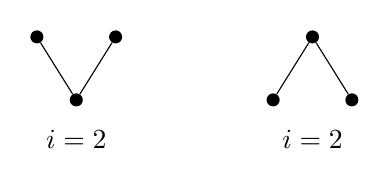
\begin{tikzpicture}
  \node[circle,fill=black,scale=0.5] (A1) at (1, 0) {};
  \node[circle,fill=black,scale=0.5] (A2) at (0.5, 0.8) {};
  \node[circle,fill=black,scale=0.5] (A3) at (1.5, 0.8) {};

  \draw (A1) -- (A2) node {};
  \draw (A1) -- (A3) node {};
  \node (AL) at (1, -0.5) {$i = 2$};


  \node[circle,fill=black,scale=0.5] (B1) at (3 + 1, 0.8) {};
  \node[circle,fill=black,scale=0.5] (B2) at (3 + 0.5, 0) {};
  \node[circle,fill=black,scale=0.5] (B3) at (3 + 1.5, 0) {};

  \draw (B1) -- (B2) node {};
  \draw (B1) -- (B3) node {};
  \node (BL) at (3 + 1, -0.5) {$i = 2$};
\end{tikzpicture}